\begin{testproblem}
(Steuerungsproblem, vgl. Beispiel~6.2.6 in \cite[S.~216~f.]{alt})\\
Es ist ein Produktionsplanungsproblem mit beschr�nktem Lager zu betrachten.
In einem Zeitraum $[0,T]$ mit $T > 0$
soll eine Produktion so gesteuert werden,
dass die Gesamtkosten minimal sind.
Seien
\begin{itemize}
  \item $z(t)$ die Anzahl der zur Zeit $t$ am Lager vorhandenen Produkte,
  \item $r(t)$ die Nachfrage nach den Produkten zur Zeit $t$ und
  \item $u(t)$ die Produktionsrate zur Zeit $t$.
\end{itemize}
Die �nderung der verf�gbaren Lagermenge $z(t)$
sei durch die Lagerbilanzgleichung
\begin{equation}
  \dot{z}(t) = u(t) - r(t) \qquad \forall t \in [0,T]
\end{equation}
mit dem Anfangslagerbestand $z(0) = a \geq 0$ gegeben.
Die Produktions- und Lagerhaltungskosten zur Zeit $t$ betragen
$\frac{1}{2} \rho_u u(t)^2 + \rho_z z(t)$
mit Konstanten $\rho_u, \rho_z > 0$.
Durch den Verkauf des Lagerrestbestandes $z(T)$
kommt ein Gewinn $\sigma z(T)$ mit $\sigma \geq 0$.
Dabei sind $u(t)$ und $z(t)$ zu bestimmen,
wobei die Lagerkapazit�t beschr�nkt ist,
d.\,h. $z(t) \leq \zeta$ f�r alle $t \in [0,T]$ mit $\zeta > 0$.
Damit ergibt sich das folgende zeitkontinuierliche Problem: 
\begin{gather}
  \min\: f(z,u) :=
    \int_0^T \left( \tfrac{1}{2} \rho_u u(t)^2 + \rho_z z(t) \right) d\!t
    - \sigma z(T) \label{prob:opt_strg_prob_produktionsplannung} \\
  \nb \quad \dot{z}(t) = u(t) - r(t) \quad \forall t \in [0,T] \notag \\
    z(0) = a \notag \\
    0 \leq z(t) \leq \zeta \quad \forall t \in [0,T] \notag \\
    0 \leq u(t) \quad \forall t \in [0,T]. \notag
\end{gather}
Eine Diskretisierung soll durchgef�hrt werden,
damit das Problem numerisch gel�st werden kann.
Mit $N \in \N$ und $\tau := \frac{T}{N}$
wird das Intervall $[0,T]$ in $N$ Teilintervalle
$[t_0,t_1], \ldots, [t_{N-1},t_N]$ unterteilt,
wobei $t_i = i\tau$ f�r alle $i = 0,\ldots,N$.
Die Produktionsrate $u(t)$ wird durch
eine st�ckweise konstante Funktion $\hat{u}(t)$ mit
\begin{equation}
  \hat{u}(t) := u_i \qquad
    \forall\, t \in [t_i, t_{i+1}[,\:
    i=0,\ldots,N-1
\end{equation}
approximiert
und die Lagermenge $z(t)$ durch
eine lineare Interpolationsfunktion $\hat{z}(t)$
mit den St�tzstellen
$(t_0,a),(t_1,z_1),\ldots,(t_N,z_N)$, d.\,h.
\begin{equation}
  \hat{z}(t) := z_i + \frac{1}{\tau}(z_{i+1} - z_i)(t - t_i) \qquad
    \forall\, t \in [t_i, t_{i+1}[, \:
    i=0,\ldots,N-1
\end{equation}
mit $z_0 := a$.
Die diskrete Version des
Problems~\eqref{prob:opt_strg_prob_produktionsplannung}
l�sst sich dann wie folgt formulieren.
\begin{gather}
  \min\: \frac{1}{2} \tau \rho_u \sum_{i=0}^{N-1} u_i^2
    + \tau \rho_z \sum_{i=1}^{N} z_i
    - \sigma z_N \label{prob:opt_strg_prob_produktionsplan_diskr}\\
  \nb \quad z_{i+1} - z_i - \tau (u_i - r_i) = 0
    \quad \forall i = 0,\ldots,N-1 \notag \\
    0 \leq z_i \leq \zeta \quad \forall i = 1,\ldots,N \notag \\
    0 \leq u_i \quad \forall i = 0,\ldots,N-1, \notag
\end{gather}
wobei $r_i := r(t_i)$ f�r $i=0,\ldots,N-1$.
Das Problem~\eqref{prob:opt_strg_prob_produktionsplan_diskr}
ist ein Problem vom Typ~\eqref{prob:quad_opt_prob_mit_lin_ungl_nebenbed}
und $x := (u_0,z_1,u_1,z_2,\ldots,u_{N-1},z_{N})^T$ sei
als die Reihenfolge der Variablen gew�hlt.
Konkrete Daten f�r den Test seien
\begin{gather}
  N = 100,\ T = 12,\ \rho_u = 0.2,\ \rho_z = 0.1,\\
  \sigma = 1.5,\ a = 5,\ \zeta = 6,\ r(t) = 10 + 5 \sin{t}.
\end{gather}
Der Startvektor $x^0 \in \R^{2N}$ sei durch
\begin{equation}
  x^0_{2i+1} := r_i, \quad x^0_{2i+2} := a
  \qquad \forall i=0,\ldots,N-1
\end{equation}
definiert.
Die Abbildung~\ref{fig:ergebnis_lagerhaltungsprob}
zeigt das Ergebnis der berechneten L�sung.
\begin{figure}[h]
\centering
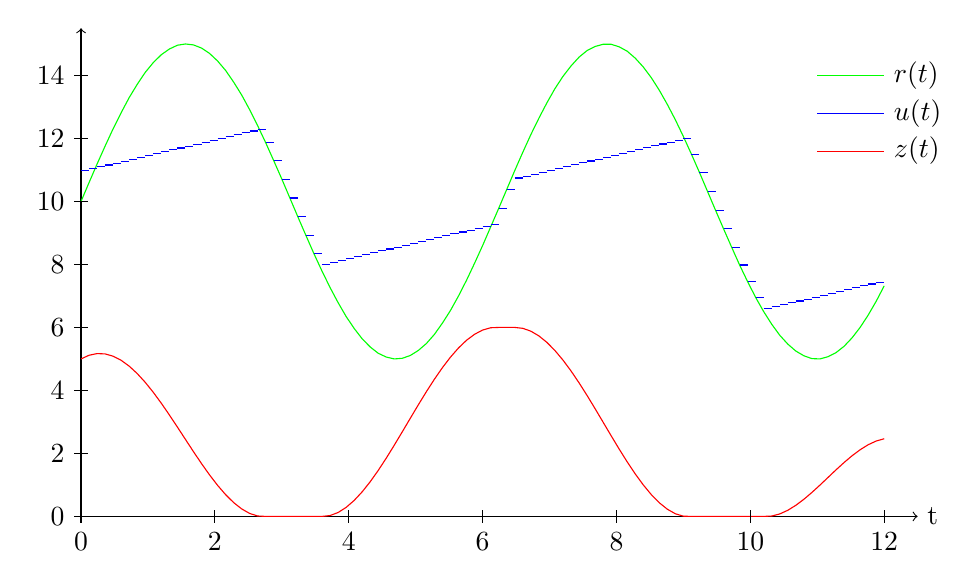
\begin{tikzpicture}[yscale=0.4,xscale=0.85]
  \draw[->] (0,0) -- (12.5,0) node [right] {t};
  \draw[->] (0,0) -- (0,15.5);
  \draw[green] (0,10) -- (0.12,10.6) -- (0.24,11.19) -- (0.36,11.76) -- (0.48,12.31) -- (0.6,12.82) -- (0.72,13.3) -- (0.84,13.72) -- (0.96,14.1) -- (1.08,14.41) -- (1.2,14.66) -- (1.32,14.84) -- (1.44,14.96) -- (1.56,15.0) -- (1.68,14.97) -- (1.8,14.87) -- (1.92,14.7) -- (2.04,14.46) -- (2.16,14.16) -- (2.28,13.79) -- (2.4,13.38) -- (2.52,12.91) -- (2.64,12.4) -- (2.76,11.86) -- (2.88,11.29) -- (3.0,10.71) -- (3.12,10.11) -- (3.24,9.51) -- (3.36,8.92) -- (3.48,8.34) -- (3.6,7.79) -- (3.72,7.27) -- (3.84,6.79) -- (3.96,6.35) -- (4.08,5.97) -- (4.2,5.64) -- (4.32,5.38) -- (4.44,5.18) -- (4.56,5.06) -- (4.68,5.0) -- (4.8,5.02) -- (4.92,5.11) -- (5.04,5.27) -- (5.16,5.49) -- (5.28,5.78) -- (5.4,6.14) -- (5.52,6.54) -- (5.64,7.0) -- (5.76,7.5) -- (5.88,8.04) -- (6.0,8.6) -- (6.12,9.19) -- (6.24,9.78) -- (6.36,10.38) -- (6.48,10.98) -- (6.6,11.56) -- (6.72,12.12) -- (6.84,12.64) -- (6.96,13.13) -- (7.08,13.58) -- (7.2,13.97) -- (7.32,14.3) -- (7.44,14.58) -- (7.56,14.79) -- (7.68,14.92) -- (7.8,14.99) -- (7.92,14.99) -- (8.04,14.91) -- (8.16,14.77) -- (8.28,14.55) -- (8.4,14.27) -- (8.52,13.93) -- (8.64,13.53) -- (8.76,13.08) -- (8.88,12.59) -- (9.0,12.06) -- (9.12,11.5) -- (9.24,10.92) -- (9.36,10.32) -- (9.48,9.72) -- (9.6,9.13) -- (9.72,8.55) -- (9.84,7.98) -- (9.96,7.45) -- (10.08,6.95) -- (10.2,6.5) -- (10.32,6.1) -- (10.44,5.75) -- (10.56,5.47) -- (10.68,5.25) -- (10.8,5.1) -- (10.92,5.01) -- (11.04,5.0) -- (11.16,5.07) -- (11.28,5.2) -- (11.4,5.4) -- (11.52,5.67) -- (11.64,6.0) -- (11.76,6.39) -- (11.88,6.83) -- (12.0,7.32);
  \foreach \x/\y in {0.0/10.977, 0.12/11.037, 0.24/11.097, 0.36/11.157, 0.48/11.217, 0.6/11.277, 0.72/11.337, 0.84/11.397, 0.96/11.457, 1.08/11.517, 1.2/11.577, 1.32/11.637, 1.44/11.697, 1.56/11.757, 1.68/11.817, 1.8/11.877, 1.92/11.937, 2.04/11.997, 2.16/12.057, 2.28/12.117, 2.4/12.177, 2.52/12.237, 2.64/12.297, 2.76/11.862, 2.88/11.293, 3.0/10.706, 3.12/10.108, 3.24/9.509, 3.36/8.917, 3.48/8.340, 3.6/8.011, 3.72/8.071, 3.84/8.131, 3.96/8.191, 4.08/8.251, 4.2/8.311, 4.32/8.371, 4.44/8.431, 4.56/8.491, 4.68/8.551, 4.8/8.611, 4.92/8.671, 5.04/8.731, 5.16/8.791, 5.28/8.851, 5.4/8.911, 5.52/8.971, 5.64/9.031, 5.76/9.091, 5.88/9.151, 6.0/9.211, 6.12/9.271, 6.24/9.784, 6.36/10.384, 6.48/10.745, 6.6/10.805, 6.72/10.865, 6.84/10.925, 6.96/10.985, 7.08/11.045, 7.2/11.105, 7.32/11.165, 7.44/11.225, 7.56/11.285, 7.68/11.345, 7.8/11.405, 7.92/11.465, 8.04/11.525, 8.16/11.585, 8.28/11.645, 8.4/11.705, 8.52/11.765, 8.64/11.825, 8.76/11.885, 8.88/11.945, 9.0/12.005, 9.12/11.500, 9.24/10.919, 9.36/10.324, 9.48/9.724, 9.6/9.128, 9.72/8.545, 9.84/7.983, 9.96/7.450, 10.08/6.953, 10.2/6.600, 10.32/6.660, 10.44/6.720, 10.56/6.780, 10.68/6.840, 10.8/6.900, 10.92/6.960, 11.04/7.020, 11.16/7.080, 11.28/7.140, 11.4/7.200, 11.52/7.260, 11.64/7.320, 11.76/7.380, 11.88/7.440}
    \draw[blue] (\x,\y) -- (\x+0.12,\y);
  \draw[red] (0,5.0) -- (0.12,5.117) -- (0.24,5.170) -- (0.36,5.159) -- (0.48,5.086) -- (0.6,4.955) -- (0.72,4.770) -- (0.84,4.534) -- (0.96,4.255) -- (1.08,3.938) -- (1.2,3.591) -- (1.32,3.221) -- (1.44,2.836) -- (1.56,2.445) -- (1.68,2.056) -- (1.8,1.677) -- (1.92,1.318) -- (2.04,0.987) -- (2.16,0.691) -- (2.28,0.439) -- (2.4,0.238) -- (2.52,0.094) -- (2.64,0.013) -- (2.76,0.000) -- (2.88,0.000) -- (3.0,0.000) -- (3.12,0.000) -- (3.24,0.000) -- (3.36,0.000) -- (3.48,0.000) -- (3.6,0.000) -- (3.72,0.027) -- (3.84,0.123) -- (3.96,0.285) -- (4.08,0.506) -- (4.2,0.780) -- (4.32,1.100) -- (4.44,1.459) -- (4.56,1.849) -- (4.68,2.261) -- (4.8,2.687) -- (4.92,3.118) -- (5.04,3.545) -- (5.16,3.961) -- (5.28,4.357) -- (5.4,4.725) -- (5.52,5.058) -- (5.64,5.349) -- (5.76,5.593) -- (5.88,5.783) -- (6.0,5.917) -- (6.12,5.990) -- (6.24,6.000) -- (6.36,6.000) -- (6.48,6.000) -- (6.6,5.972) -- (6.72,5.882) -- (6.84,5.732) -- (6.96,5.526) -- (7.08,5.268) -- (7.2,4.964) -- (7.32,4.621) -- (7.44,4.244) -- (7.56,3.842) -- (7.68,3.422) -- (7.8,2.992) -- (7.92,2.562) -- (8.04,2.139) -- (8.16,1.732) -- (8.28,1.350) -- (8.4,1.001) -- (8.52,0.693) -- (8.64,0.433) -- (8.76,0.228) -- (8.88,0.084) -- (9.0,0.007) -- (9.12,0.000) -- (9.24,0.000) -- (9.36,0.000) -- (9.48,0.000) -- (9.6,0.000) -- (9.72,0.000) -- (9.84,0.000) -- (9.96,0.000) -- (10.08,0.000) -- (10.2,0.000) -- (10.32,0.012) -- (10.44,0.079) -- (10.56,0.195) -- (10.68,0.353) -- (10.8,0.544) -- (10.92,0.761) -- (11.04,0.994) -- (11.16,1.236) -- (11.28,1.478) -- (11.4,1.710) -- (11.52,1.926) -- (11.64,2.116) -- (11.76,2.275) -- (11.88,2.393) -- (12.0,2.466);
  \foreach \x in {0,2,...,12}
    \draw (\x,0.2) -- (\x,-0.2) node [below] {\x};
  \foreach \y in {0,2,...,14}
    \draw (0.1,\y) -- (-0.1,\y) node [left] {\y};
  \draw[green] (11,14) -- (12,14) node [black,right] {$r(t)$};
  \draw[blue] (11,12.8) -- (12,12.8) node [black,right] {$u(t)$};
  \draw[red] (11,11.6) -- (12,11.6) node [black,right] {$z(t)$};
\end{tikzpicture}
\caption{Ergebnis des
Produktionsplanungsproblems~\ref{prob:opt_strg_prob_produktionsplan_diskr}}
\label{fig:ergebnis_lagerhaltungsprob}
\end{figure}
\end{testproblem}